%!TEX spellcheck = fr_FR
%!TEX encoding = UTF-8 Unicode
%!TEX TS-program = xelatex

\documentclass[xcolor=dvipsnames, 10pt, french, american]{beamer} 

% —  —  —  —  —  —  —  —  —  —  —  —  —  —  —  —  —  —  —  — 
% 			CHARGEMENT PACKAGES					%
% —  —  —  —  —  —  —  —  —  —  —  —  —  —  —  —  —  —  —  — 

\usepackage{libertine}
\usepackage{courier}
\usepackage{babel}
\usepackage{xspace}
\usepackage{xcolor}
\usepackage{csquotes}


\hypersetup{
  colorlinks,
  allcolors=.,
  urlcolor=magenta,
  pdftitle={},
  pdfauthor={CAA-FR},
  pdfsubject={},%
  pdfkeywords={},%
 pdfcreator={LuaLaTeX},%
}
 

 

% —  —  —  —  —  —  —  —  —  —  —  —  —  —  —  —  —  —  —  — 
% 			CONFIGURATION BEAMER					%
% —  —  —  —  —  —  —  —  —  —  —  —  —  —  —  —  —  —  —  — 

 \usetheme{Antibes}%Berlin, Warsaw, Copenhagen, Frankfurt, Antibes  Darmstadt
%\usecolortheme{crane}% crane seagull
\usecolortheme[named=Violet]{structure} %  Aquamarine RawSienna RedViolet    WildStrawberry  Magenta Turquoise YellowGreen    dvipsnam.def  pour la liste de couleurs
%~ \usefonttheme{structuresmallcapsserif}
\setbeamertemplate{background canvas}[verticalshading, top=couleur1, middle=couleur2, midpoint=valeur, bottom=couleur3,  bibliography item=triangle]
\setbeamerfont{headline}{size=\normalsize, }
\setbeamerfont{frametitle}{size=\large, }

\beamertemplatenavigationsymbolsempty
\setcounter{secnumdepth}{1}% profondeur jusqu'à ce que les sections sont numérotées (partie=-1 ; chapitre=0 ; section=1 ; subsection=2)
\setcounter{tocdepth}{2}%profondeur jusqu'à laquelle elles sont affichées dans la TOC


% — 

% —  —  —  —  —  —  —  —  —  —  —  —  —  —  —  —  —  —  
% 			DONNÉES DESCRIPTIVES					%
% —  —  —  —  —  —  —  —  —  —  —  —  —  —  —  —  —  —  


%================================================
%	TITLE PAGE
%================================================
\title{CAA-FR, the French CAA chapter} 
\subtitle{Computer Applications and Quantitative Methods in Archaeology}

\author{\url{https://caafrance.hypotheses.org}}
% \institute{}

\date{GMPCA 2025, Rouen, 14 avril 2025\\\bigskip


\includegraphics[height=0.1\textheight]{figures/caa-fr-logo.png}
}

%================================================
%	BEGIN DOCUMENT 
%================================================
\begin{document}

%------------------------------------------------
%	TITLE SLIDE
%------------------------------------------------
\begin{frame}
    \titlepage
\end{frame}


\section{CAA International}
\frame{\tableofcontents[sectionstyle=show/shaded, subsectionstyle=show/hide/hide]}
 
 
 \begin{frame}
    \begin{block}{What is the CAA International?}
    
        Computer Applications and Quantitative Methods in Archaeology\medskip
        
        \begin{quote}
            CAA is an international organisation bringing together archaeologists, mathematicians and computer scientists. Its aims are to encourage communication between these disciplines, to provide a survey of present work in the field and to stimulate discussion and future progress.
        \end{quote}
        
        \url{https://caa-international.org}
    \end{block}
 \end{frame}
 
 
 
\begin{frame}
    \begin{block}{Special Interest Groups}
        \begin{itemize}
            \item    Complex Systems Simulation
            \item     Computer Programs for Archaeologists
            \item Mobile GIS
            \item     3D spatial analysis
            \item     Scientific Scripting Languages in Archaeology (SIG-SSLA)
            \item Semantics and LOUD in Archaeology (SIG Data-Dragon)
            \item Archaeological Practices and Knowledge Work (SIG ARKWORK)
            \item Computationally Modeling Water-based Movement (SIG CMWM)
        \end{itemize}
    \end{block}
\end{frame}
    
 

\begin{frame}
    \centering
        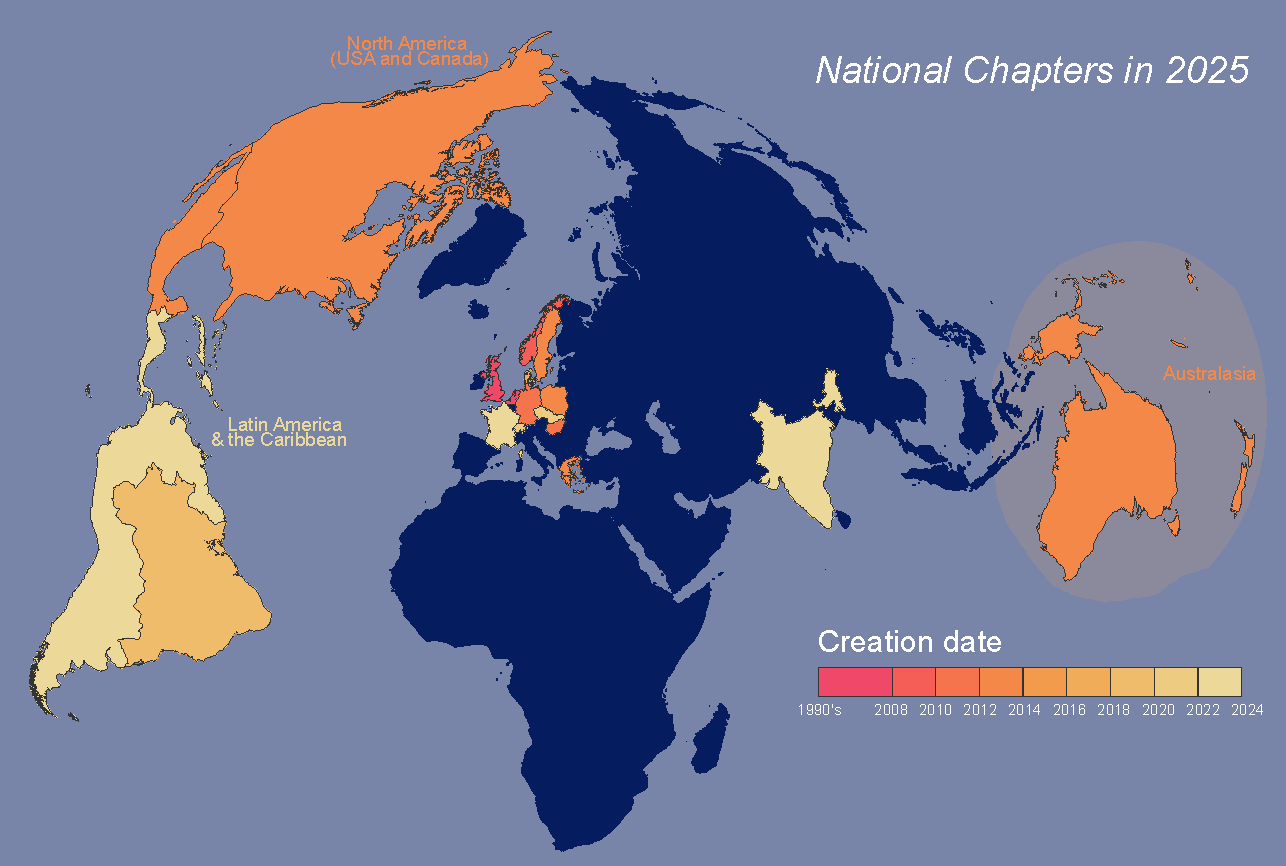
\includegraphics[height=0.8\textheight]{figures/national-chapters2025}
\end{frame}



\section{Overview of the CAA-FR} 
\frame{\tableofcontents[sectionstyle=show/shaded, subsectionstyle=show/hide/hide]}
 

\begin{frame}
    \begin{block}{Creation}
        \only<2>{
            CAA-FR was created at the CAA 2024 Auckland conference!
        
            \begin{center}
                
\includegraphics[height=0.3\textheight]{figures/caa2024}      
            \end{center}
        }
    \end{block}
    
    \begin{block}{Objectives}
        \only<3>{
            \begin{itemize}
                \item To bring together archaeologists, archaeometrists, mathematicians, computer scientists and members of other disciplines based in France to complement and extend the interests of CAA International.
                \item To encourage communication between these disciplines.
                \item To give a survey of present work in the field.
                \item To stimulate discussion and future progress in the application of information technology to archaeological research and practice.
                \item To provide guidance and support in the form of seminars and/or workshops.
            \end{itemize}
        }
    \end{block}
\end{frame}
    

\begin{frame}
    \begin{block}{Current \textit{Bureau}}
        \begin{itemize}
            \item \textbf{2024-2025} \& an election biennially at the CAA-FR General Meeting % je ne comprnds pas ce que ça veut dire
            \item \textbf{Three speakers}:
                \begin{itemize}
                    \item Dr Nicolas Frerebeau (UMR 6034 Archéosciences Bordeaux)
                    \item Dr Gwénaëlle Moreau (SpaceARC) % j'ai fait du copier-coller, si ça tient à moi > je virerai le "Dr"
                    \item Dr Sébastien Plutniak (UMR 7324 CITERES, Tours)
                \end{itemize}
            \item \textbf{Three vice-speakers}:
                \begin{itemize}
                    \item Dr Anaïs Vignoles (MSCA fellow, Université de Liège)
                    \item Mathias Bellat (PhD candidate, University of Tübingen) 
                    \item Dr Julie Gravier (UMR 6049 ThéMA, Besançon)
                \end{itemize}
        \end{itemize}
    \end{block}
\end{frame}


\section{Activities since 2024}
\frame{\tableofcontents[sectionstyle=show/shaded, subsectionstyle=show/hide/hide]}
 

\subsection{Online presence}
\frame{\tableofcontents[sectionstyle=show/shaded, subsectionstyle=show/shaded/hide]}
 
 
\begin{frame}
	\begin{block}{CAA-FR Website}
        \begin{center}
            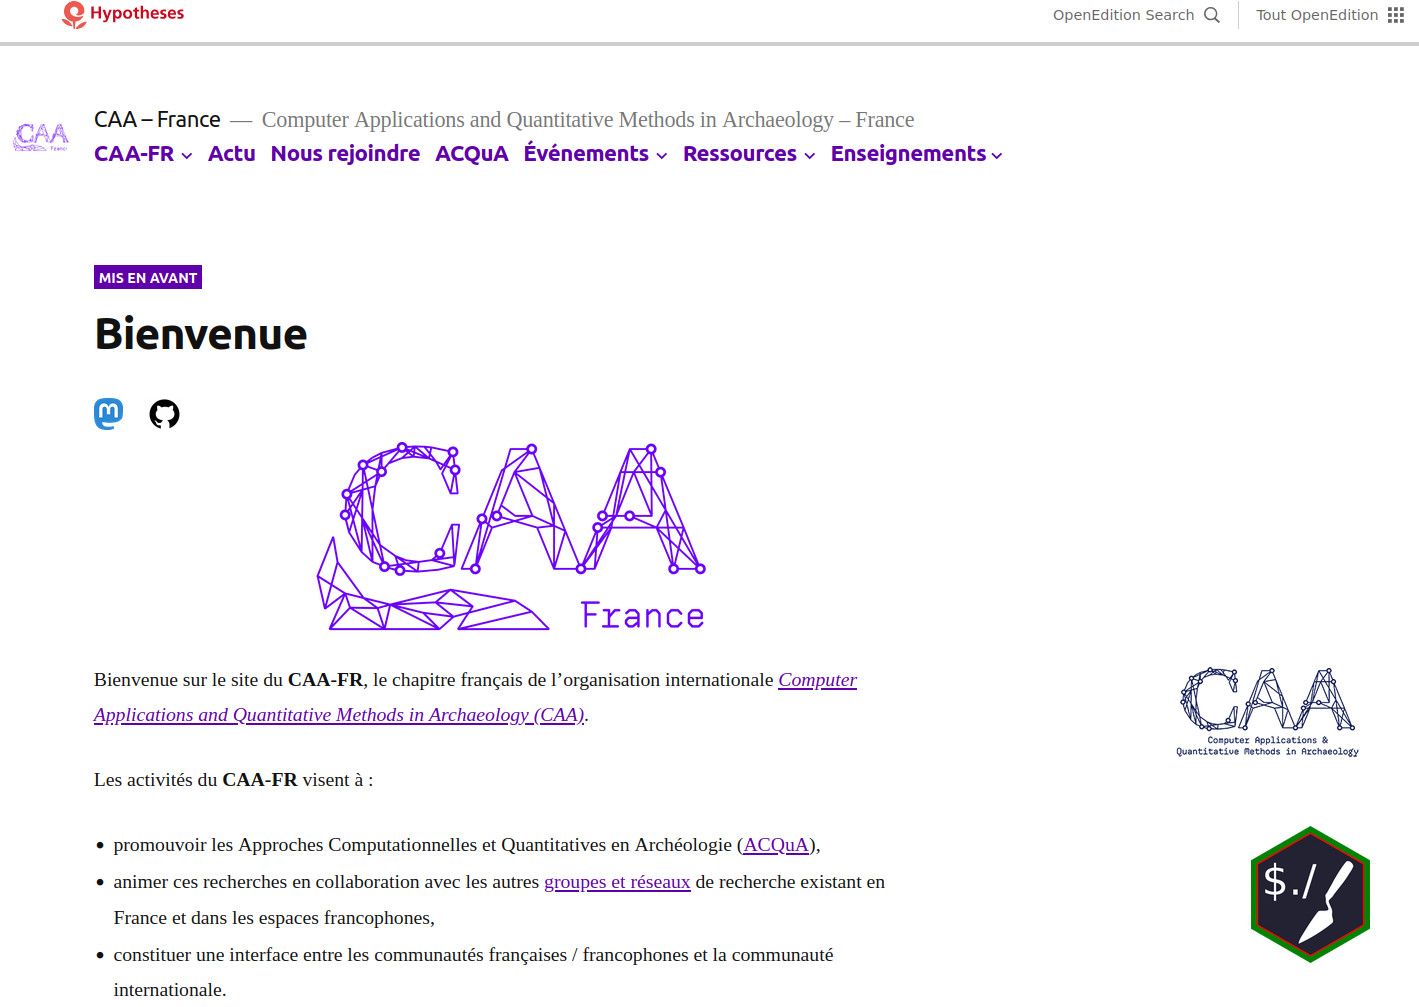
\includegraphics[height=0.6\textheight]{figures/caa-fr-website}
        \end{center}
        \url{https://caafrance.hypotheses.org}
	\end{block}
\end{frame}


\begin{frame}
     \begin{columns}[t]
    	\column{0.5\textwidth}
            CAA-FR \emph{Mastodon} account\medskip
            
            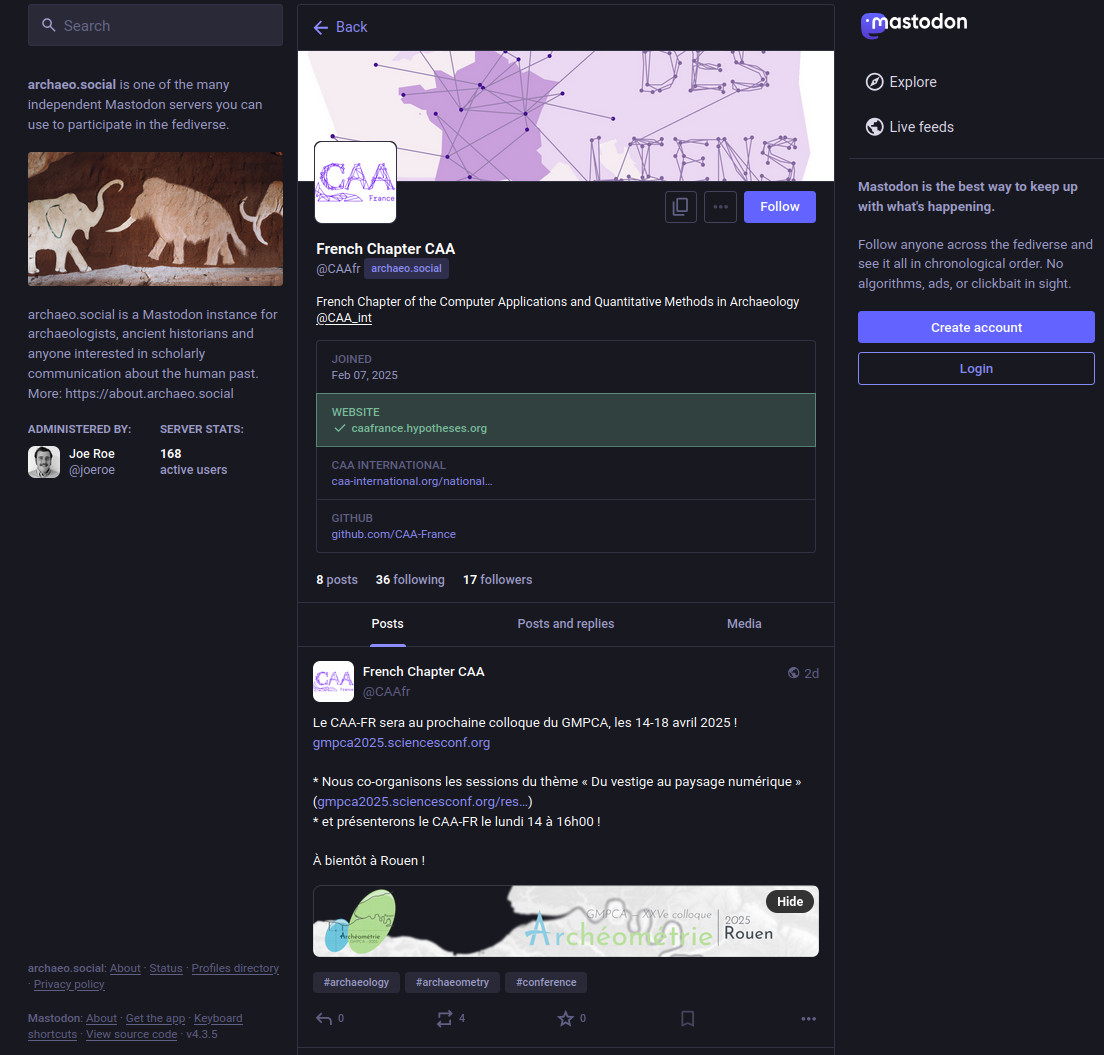
\includegraphics[height=0.5\textheight]{figures/caa-fr-mastodon}\medskip
            
            \url{https://archaeo.social/@CAAfr}
    	
    	\column{0.5\textwidth}
            CAA-FR \emph{github} repositories\medskip
            
            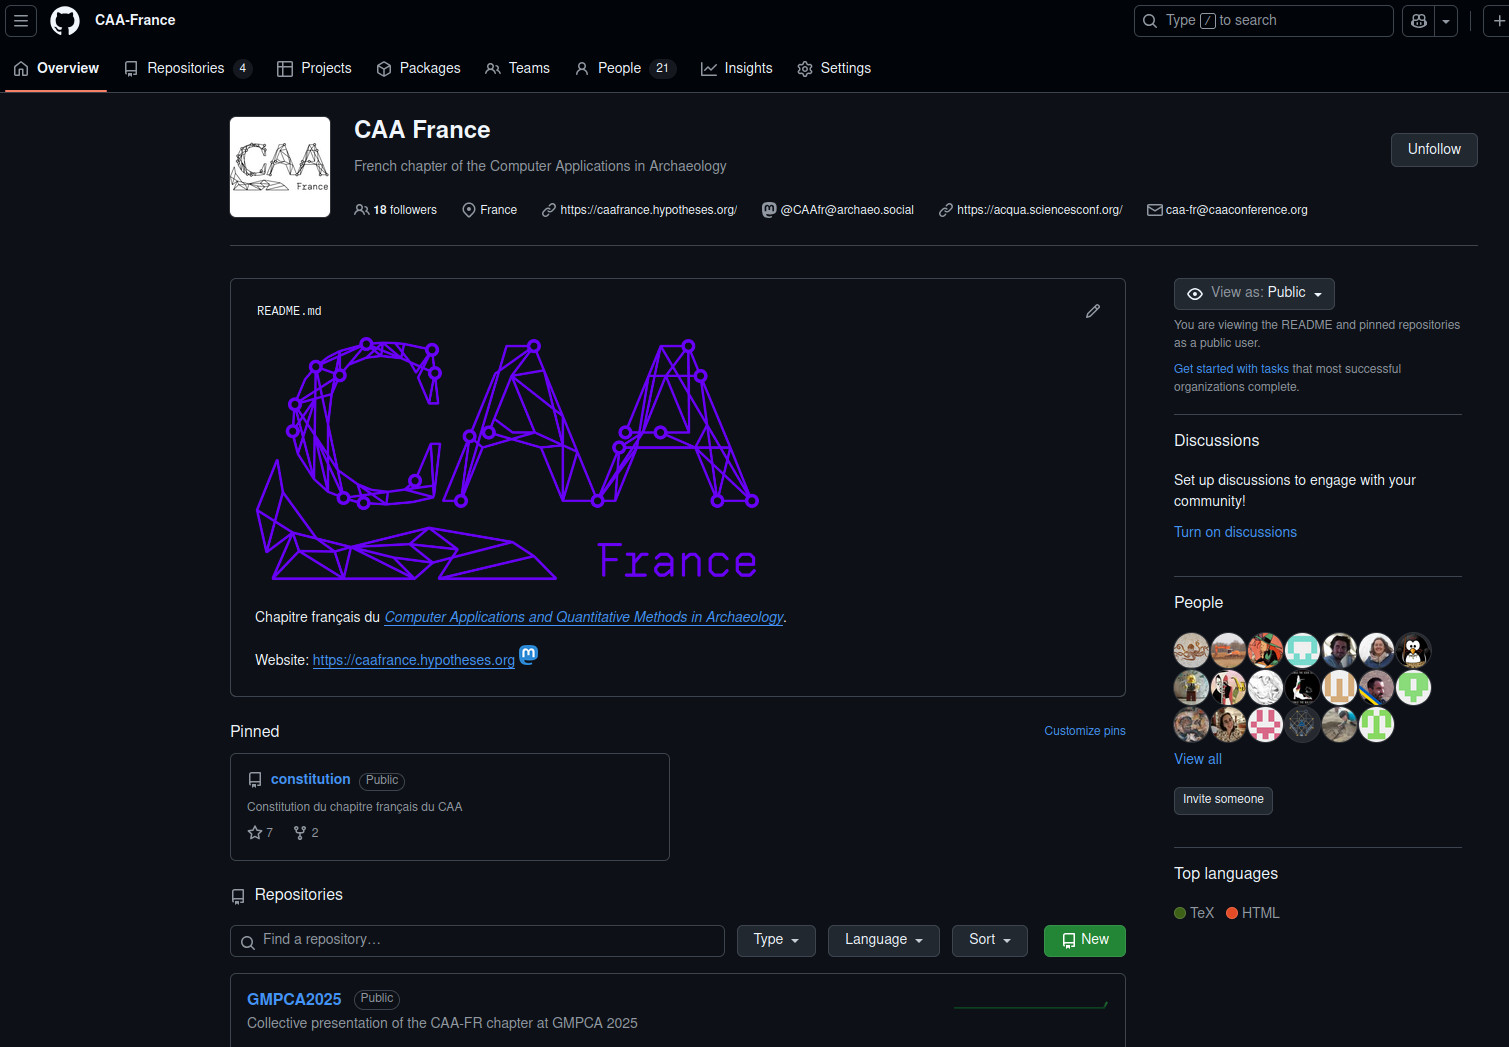
\includegraphics[height=0.5\textheight]{figures/caa-fr-github}\medskip
            
            \url{https://github.com/CAA-France}
    \end{columns}
\end{frame}



\subsection{The \emph{ACQuA} launching conference}
\frame{\tableofcontents[sectionstyle=show/shaded, subsectionstyle=show/shaded/hide]}
 

\begin{frame}

    \url{https://acqua.sciencesconf.org}
    
    \begin{columns}[t]
    	
    	\column{0.5\textwidth}
    	
        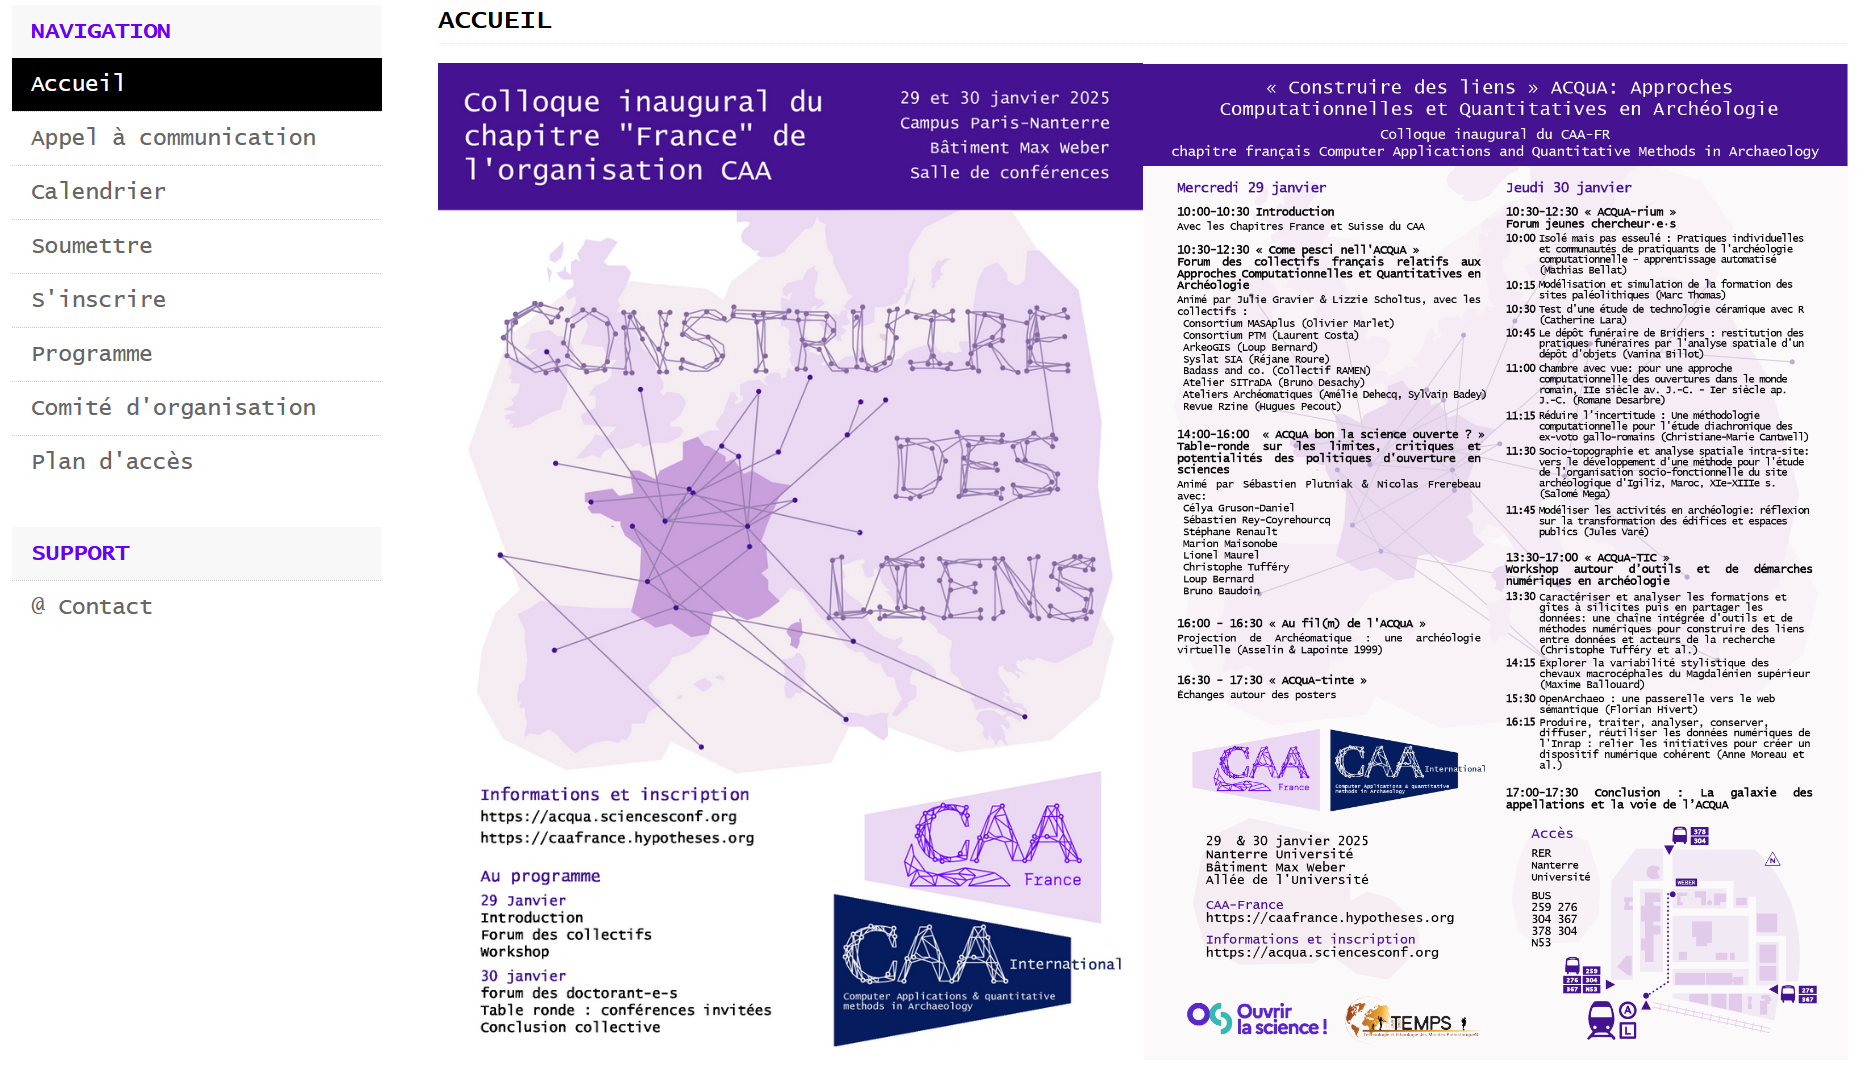
\includegraphics[height=0.4\textheight]{figures/acqua2025}
    	
    	\column{0.5\textwidth}
    	
    	\textbf{4 formats}
    	
    	\begin{itemize}
    		\item Forum of French collectives % Forum des collectifs français : 8 collectifs
    		\item Round table on the limits, criticisms and potential of open sciences policies % Table-ronde sur les limites, critiques et potentialités des politiques d'ouverture en sciences > 8 invités
    		\item Forum of young researchers % Forum des jeunes chercheur·e·s présentations flashs > 8 présentations
    		\item Workshop on digital tools and approaches in archaeology % Workshop autour d'outils et de démarches numériques en archéologie > 4 présentations plus longues avec envoi de textes préalablement au workshop
    	\end{itemize}
    \end{columns}
\end{frame}


\begin{frame}
    \begin{center}
        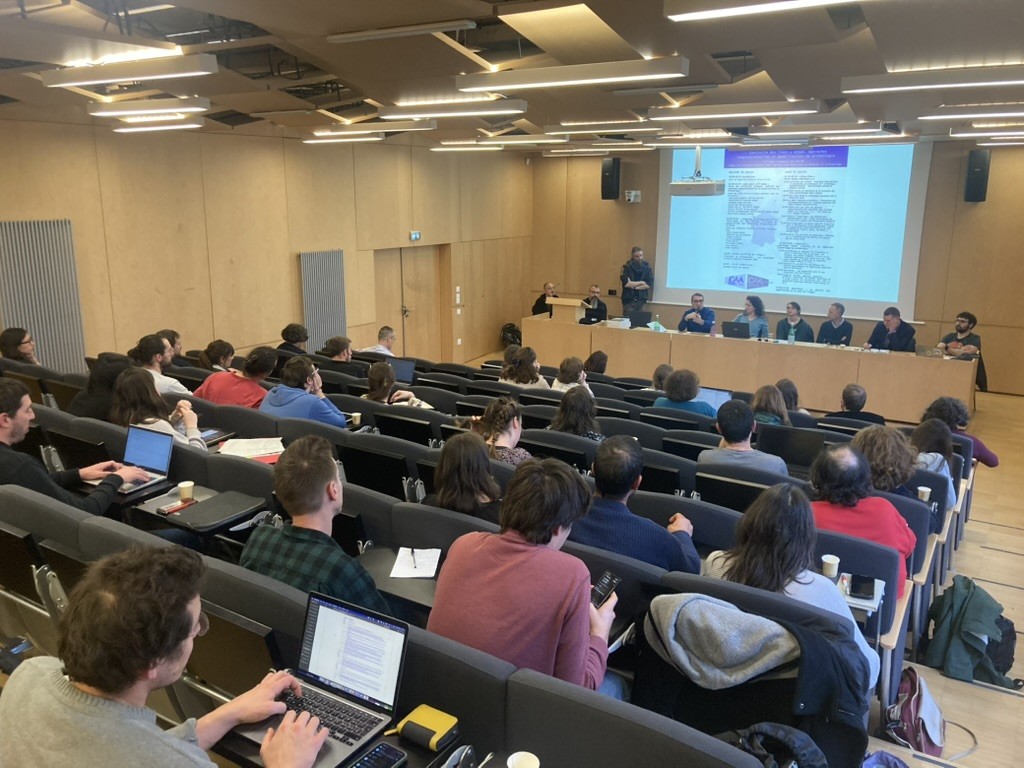
\includegraphics[height=0.45\textheight]{figures/acqua1}
        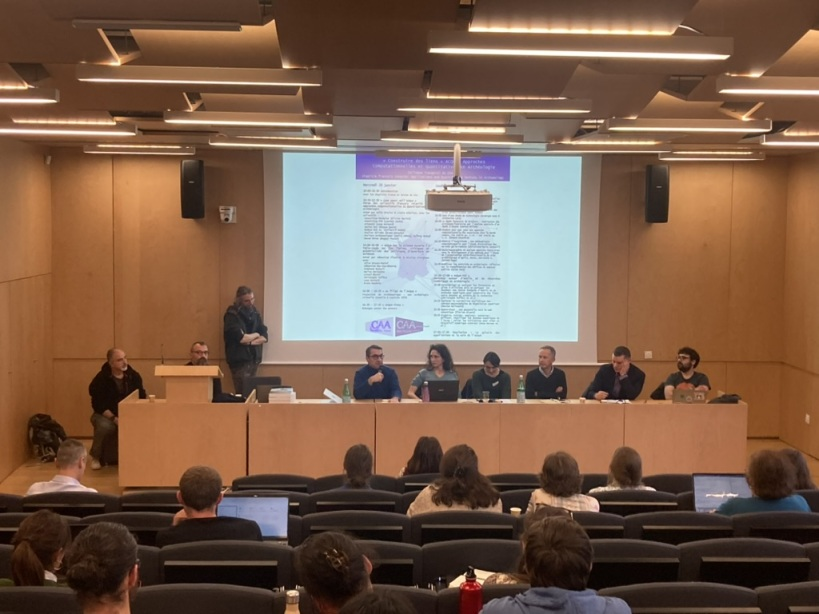
\includegraphics[height=0.45\textheight]{figures/acqua2}
    \end{center}
\end{frame}


\begin{frame}
    \begin{center}
        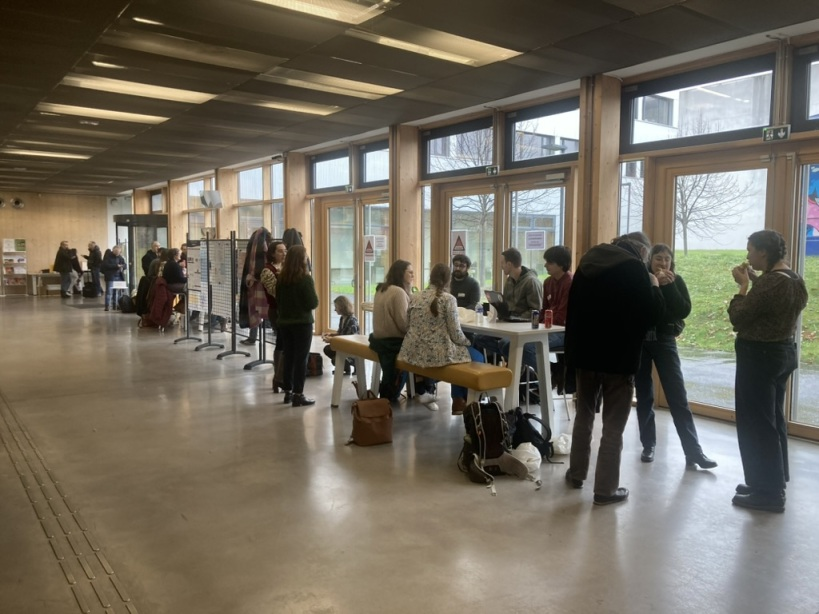
\includegraphics[height=0.6\textheight]{figures/acqua3}
        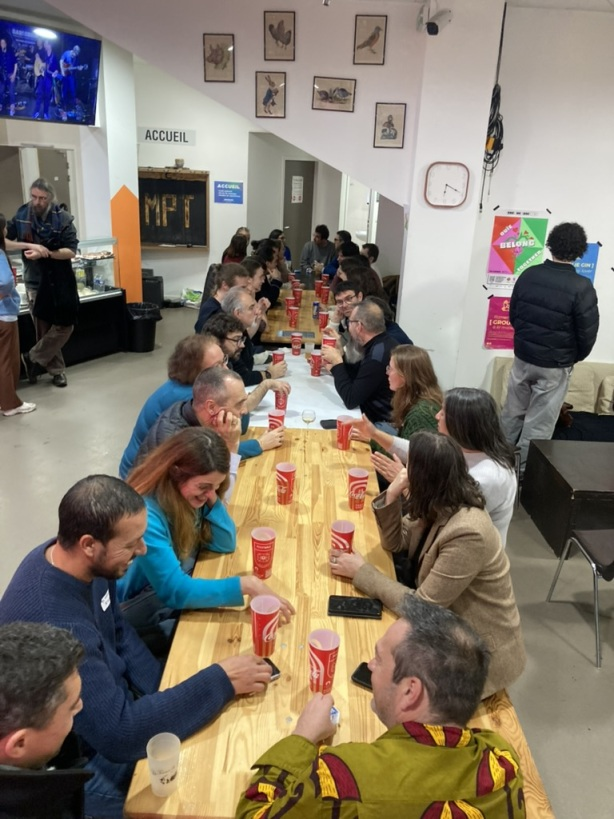
\includegraphics[height=0.6\textheight]{figures/acqua4}
    \end{center}
\end{frame}




\subsection{Other actions}
\frame{\tableofcontents[sectionstyle=show/shaded, subsectionstyle=show/shaded/hide]}
 
 
\begin{frame}
    \begin{block}{\textbf{Support for young researchers for CAA Athens 2025}}
       
        \begin{itemize}
            \item In collaboration with the École française d'Athènes
            \item 5 rooms available during the week of the conference 
        \end{itemize}
    \end{block}
\end{frame}



\section{Join us!}
\frame{\tableofcontents[sectionstyle=show/shaded, subsectionstyle=show/hide/hide]}
 
 
\begin{frame}
	\begin{block}{Two mailing lists}
		\begin{itemize}
			\item \textbf{To become a member} of the chapter: \\
                \url{https://framagroupes.org/sympa/info/caa.france}\\
                 34 subscribers (April 2025)
			\item \textbf{To receive information} about the chapter's activities (without becoming a member):\\ 
                \url{https://framagroupes.org/sympa/info/caa.france.info}\\
                  54 subscribers (April 2025)
		\end{itemize}
	\end{block}
\end{frame}

\end{document}
